

\begin{frame}
\frametitle{Brainteaser 1}
When the system shown in Figure (a) is subjected to a unit-step input, the system output responds as shown in Figure (b)
\\Determine the values of K and T from the response curve.
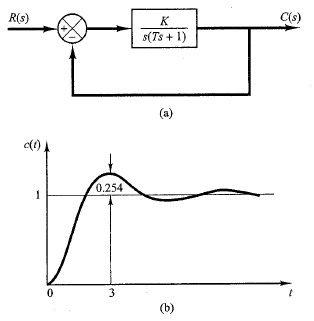
\includegraphics[width=0.5\linewidth]{Afbeelding1}
\end{frame}

\begin{frame}
\frametitle{Solution 1}
The maximum overshoot of $0.254$ corresponds to $\zeta = 0.4$.
\\From the response curve we have $t_p = 3$
\Consequently, $t_p = \fraq{\pi}{\omega_d} = \frac{\pi}{\omega_n\sqrt{1-\zeta^2}} = 3$
\\It follows that $ \omega_n =1.14$
\\From the block diagram we have $\frac{C(s)}{R(s)} = \frac{K}{Ts^2 + s + K}$
\\from which $\omega_n = \sqrt{\frac{K}{T}}$, $2\zeta\omega_n = \frac{1}{T}$
\\ Therefore, the values of T and K are determined as
\\ $T = \frac{1}{2\zeta\omega_n} = \frac{1}{2 x 0.4 x 1.14} = 1.09$
\\ $K = \omega_n ^2 T = 1.14^2 x 1.09 = 1.42$
\\ Source: Ogata, Modern Control Engineering 4th edition, p.$298$ 
\end{frame}

\begin{frame}{Brainteaser 2}
\\ Two linear, time invariant systems are connected in series. 
\\ For a periodic input $u(t) = sin(\alpha t)$, 
\\ is $y_{ss}= |H_1(j\alpha)||H_2(j\alpha)|sin(\alpha t +	\angle H_1(j\alpha) + H_2(j\alpha))$ the steady state output ?
\end{frame}

\begin{frame}{Solution 2}
Old exam question, answer should be around
\end{frame}

\begin{frame}{Brainteaser 3}
We have found the step-response of a physical system with 1 input and 1 output. This response converges to a constant value. Can we conclude that the system is internal stable? 
\end{frame}

\begin{frame}
Old exam question, answer should be around.
\end{frame} 

\begin{frame}{Brainteaser 4}
Find the laplace transformation of
\begin{cases}

f(t)=0  &t<0
\\f(t)=sin(\omega t+\theta)& t\ge 0

\end{cases}
\end{frame}

\begin{frame}{Solution 4}
Noting that $sin(\omega t +\theta) = sin(\omega t)cos(\theta) + cos(\omega t)sin(\theta)$
\\We have $\mathcal{L}\big[sin(\omega t + \theta)\big] =
cos(\theta)\mathcal{L}\big[sin(\omega t)\big] + sin(\theta)\mathcal{L}\big[cos(\omega t)\big]=
 \frac{\omega cos(\theta) +  sin(\theta)s }{s^2+\omega^2}$
\end{frame}